\documentclass[aspectratio=169]{beamer}

\usepackage[T2A,T1]{fontenc}
\usepackage[utf8]{inputenc}
\usepackage[english,russian]{babel}
\usepackage{amsmath}
\usepackage{amssymb}
\usepackage{booktabs}
\usepackage{multirow}
\usepackage{graphicx}

\usetheme{default}
\usecolortheme{default}
\usefonttheme{default}

\setbeamercolor{background canvas}{bg=white}
\setbeamercolor{normal text}{fg=black}
\setbeamercolor{frametitle}{fg=black,bg=white}
\setbeamercolor{title}{fg=black}
\setbeamercolor{author}{fg=black}
\setbeamercolor{institute}{fg=black}
\setbeamercolor{date}{fg=black}
\setbeamercolor{itemize item}{fg=black}
\setbeamercolor{itemize subitem}{fg=black}
\setbeamercolor{enumerate item}{fg=black}
\setbeamercolor{block title}{fg=black,bg=white}
\setbeamercolor{block body}{fg=black,bg=white}
\setbeamercolor{section in toc}{fg=black}

\setbeamertemplate{navigation symbols}{}
\setbeamertemplate{itemize item}{--}
\setbeamertemplate{itemize subitem}{--}

% Разделитель под заголовком слайда
\setbeamertemplate{frametitle}{%
  \vspace{0.6em}%
  \insertframetitle\strut%
  \vspace{0.15em}%
  \hrule height 0.4pt%
  \vspace{0.4em}%
}

% Минимальный футер: только номер слайда справа
\setbeamertemplate{footline}{%
  \hfill%
  \usebeamerfont{footline}\insertframenumber%
  \hspace{1em}\vspace{0.5em}%
}

\setbeamertemplate{blocks}[default]

\title[Детекция дефектов речи]{Детекция дефектов речи с помощью скороговорок}
\author{Кузьмин Дмитрий Андреевич}
\institute{%
  Факультет компьютерных наук НИУ ВШЭ\\
  Программа «Искусственный интеллект»\\[2em]
  Научный руководитель: Кантонистова Елена Олеговна\\
  Соруководитель: Ковалева Александра Ивановна
}
\date{Москва, 2026}

\begin{document}

% ── Слайд 1. Титульный ──────────────────────────────────────────────────────
\begin{frame}
  \vfill
  \centering
  {\large\textbf{\inserttitle}}\\[1.2em]
  {\normalsize\insertauthor}\\[2em]
  {\small\insertinstitute}
  \vfill
  {\small\insertdate}
\end{frame}

% ── Слайд 2. Мотивация ──────────────────────────────────────────────────────
\begin{frame}{Мотивация}
  \begin{columns}[T]
    \column{0.55\textwidth}
      \textbf{Проблема}
      \begin{itemize}
        \item Нарушения речи у детей влияют на обучение и социальную адаптацию
        \item Диагностика требует оценки логопеда
        \item Регулярный мониторинг динамики
      \end{itemize}
      \vspace{0.8em}
      
    \column{0.42\textwidth}
      \textbf{Типы причин дефектов речи}\\[0.5em]
      \begin{itemize}
        \item недоразвитость речевого аппарата;
        \item поражение нервной системы (дизартрия, афазия и др.);
        \item дефекты речевого аппарата (ринолалия и др.).
      \end{itemize}
  \end{columns}
  \textbf{Решение}
      \begin{itemize}
        \item Автоматическая система с возможностью контроля динамики
        \item Скороговорки - лучший способ выявления
      \end{itemize}
\end{frame}

% ── Слайд 3. Постановка задачи ──────────────────────────────────────────────
\begin{frame}{Постановка задачи}
  \begin{itemize}
    \item \textbf{Тип задачи:} бинарная классификация аудиозаписей детской речи
    \item \textbf{Вход:} аудиофайл чтения скороговорки $x_i$;\quad \textbf{выход:} $y_i \in \{0, 1\}$
    \item \textbf{Классы:} \textbf{good} (нормальное произношение), \textbf{bad} (наличие речевого дефекта)
    \item \textbf{Прикладная цель:} Telegram-бот для мониторинга динамики
  \end{itemize}
\end{frame}

% ── Слайд 4. Датасет ────────────────────────────────────────────────────────
\begin{frame}{Описание датасета}
  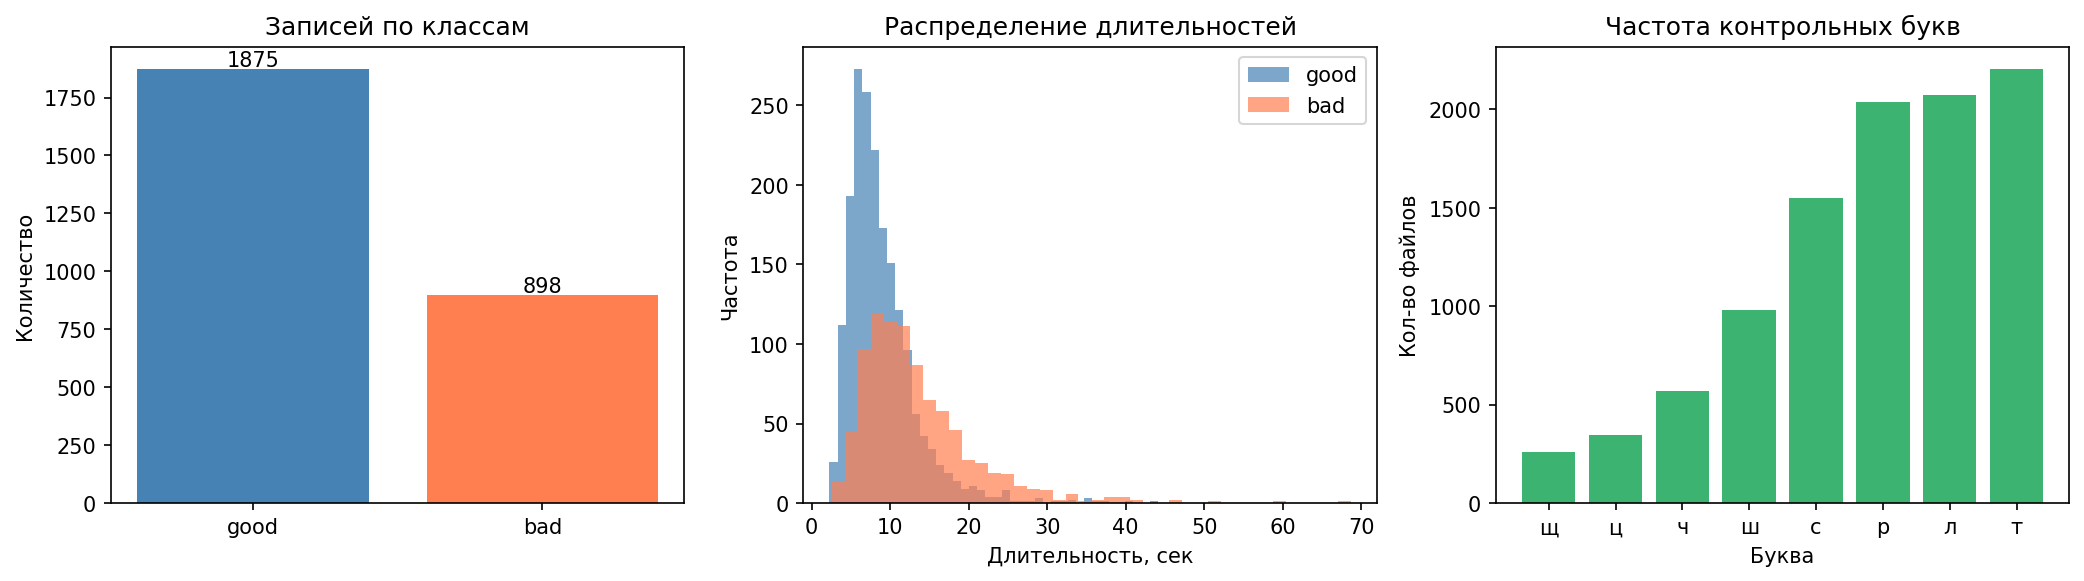
\includegraphics[width=\textwidth]{../../experiments/dataset_overview.png}

  \begin{columns}[T]
    \column{0.48\textwidth}
      \textbf{Ключевые особенности:}
      \begin{itemize}
        \item Малый объём (2773 записи)
        \item Дисбаланс классов (2/3 — good)
        \item Каждая запись помечена ${\geq}1$ контрольной буквой \\ (т, л, р, с, ш, ч, ц, щ)
      \end{itemize}
    \column{0.48\textwidth}
      \textbf{Длительность аудио (сек.)}
      \begin{tabular}{lcccc}
        \toprule
         & min & max & mean & median \\
        \midrule
        good & 2.28 & 44.10 & 8.89 & 7.86 \\
        bad  & 2.62 & 68.66 & 13.47 & 11.84 \\
        all  & 2.28 & 68.66 & 10.37 & 8.86 \\
        \bottomrule
      \end{tabular}
  \end{columns}
\end{frame}

% ── Слайд 5. Метрики ────────────────────────────────────────────────────────
\begin{frame}{Метрики оценки качества}
  \textbf{Иерархия важности метрик:}
  \begin{enumerate}
    \item $\mathbf{F1_{\text{bad}}}$ — ключевая (не пропустить дефект)
    \item \normalsize $F1_{\text{macro}}$ — баланс по классам
    \item Accuracy — общий индикатор
  \end{enumerate}
\end{frame}

% ── Слайд 6. Группа 1: Классические ML ─────────────────────────────────────
\begin{frame}{Группа 1: Классические ML-модели}
  \textbf{Результаты:}\\[0.3em]
  \begin{tabular}{lccc}
    \toprule
    \textbf{Модель} & \textbf{F1-bad} & \textbf{F1-macro} & \textbf{Acc} \\
    \midrule
    MFCC + RF           & 0.540 & 0.679 & 0.739 \\
    \textbf{VGGish + SVM}        & \textbf{0.597} & \textbf{0.692} & \textbf{0.722} \\
    \bottomrule
  \end{tabular}
\end{frame}

% ── Слайд 7: Группа 2: DL на спектрограммах ────────────────────────────────
\begin{frame}{Группа 2: Нейронные сети на спектрограммах}
  \textbf{Результаты:}\\[0.3em]
  \setlength{\tabcolsep}{4pt}
  \begin{tabular}{lccc}
    \toprule
    \textbf{Модель} & \textbf{F1-bad} & \textbf{F1-macro} & \textbf{Acc} \\
    \midrule
    1D CNN (waveform)        & 0.561 & 0.689 & 0.741 \\
    2D CNN (log-mel)         & 0.567 & 0.673 & 0.707 \\
    BiLSTM (MFCC)            & 0.530 & 0.656 & 0.703 \\
    Swin Tiny (mel)          & 0.597 & 0.718 & 0.770 \\
    \textbf{DSSCNet}         & \textbf{0.624} & \textbf{0.716} & \textbf{0.746} \\
    FluentNet                & 0.610 & 0.686 & 0.705 \\
    \bottomrule
  \end{tabular}
\end{frame}

% ── Слайд 8: Группа 3: Предобученные эмбеддинги ────────────────────────────
\begin{frame}{Группа 3: Предобученные речевые эмбеддинги}
  \textbf{Результаты:}\\[0.2em]
  \setlength{\tabcolsep}{4pt}
  \begin{tabular}{lccc}
    \toprule
    \textbf{Модель} & \textbf{F1-bad} & \textbf{F1-macro} & \textbf{Acc} \\
    \midrule
    Wav2Vec2 + SVM                    & 0.617 & 0.717 & 0.753 \\
    HuBERT + SVM                     & 0.628 & 0.745 & 0.799 \\
    OpenL3 + SVM                      & 0.664 & 0.750 & 0.779 \\
    XLS-R + SVM                       & 0.642 & 0.747 & 0.791 \\
    Whisper-small + SVM               & 0.722 & 0.799 & 0.830 \\
    \textbf{Whisper-med + SVM}        & \textbf{0.747} & \textbf{0.815} & \textbf{0.839} \\
    Whisper-large + SVM               & 0.724 & 0.802 & 0.832 \\
    Whisper-special + SVM             & 0.644 & 0.751 & 0.796 \\
    \bottomrule
  \end{tabular}
\end{frame}


% ── Слайд 11: Улучшения пайплайна в experiments/ ────────────────────────────
\begin{frame}{Улучшения пайплайна}
  \footnotesize
  \setlength{\tabcolsep}{5pt}
  \begin{tabular}{p{0.28\textwidth}p{0.32\textwidth}p{0.32\textwidth}}
    \toprule
    \textbf{Аспект} & \textbf{Текущий пайплайн} & \textbf{Улучшения} \\
    \midrule
    CV & Один сплит & 5-fold Stratified CV на train+val \\[0.4em]
    Порог & 0.5 фиксированный & Оптимальный для максимума F1-bad на val\\[0.4em]
    Аугментация & Нет & Планируется \\[0.4em]
    \bottomrule
  \end{tabular}
\end{frame}

% ── Слайд 11: Заключение ────────────────────────────────────────────────────
\begin{frame}{Заключение}
  \textbf{Ключевой вывод:}\\
  Предобученные речевые модели (Whisper, HuBERT) обеспечивают наилучшую детекцию дефектов речи при малом объёме данных \\[1em]

  \textbf{Дальнейшие шаги:}
  \begin{itemize}
    \item Fine-tuning предобученных моделей
    \item Аугментация для DL моделей
    \item Мультиклассовая постановка (по типу дефекта)
    \item Написание сервиса (Telegram-бота) для мониторинга динамики
  \end{itemize}
\end{frame}

% ── Слайд 12: Спасибо ───────────────────────────────────────────────────────
\begin{frame}
  \vfill
  \centering
  {\LARGE Спасибо за внимание}
  \vfill
\end{frame}

\end{document}
